\documentclass[chaptersright]{informeutn}
\usepackage[table]{xcolor}
\usepackage{array}
\usepackage{tikz/tikzit}
\usepackage{listings}

\input{tikz/TikZiT_style.tikzstyles}

\lstdefinestyle{ltspice}{
  backgroundcolor=\color{gray!10},
  basicstyle=\ttfamily\small,
  keywordstyle=\color{blue},
  commentstyle=\color{green!50!black},
  stringstyle=\color{orange},
  frame=single,
  breaklines=true,
  postbreak=\mbox{\textcolor{red}{$\hookrightarrow$}\space},
  columns=flexible,
  captionpos=b
}
\renewcommand{\lstlistingname}{Listado}

% Datos del informe
\materia{Dispositivos Electrónicos}
\titulo{Trabajo Práctico 4}
\comision{3R2}
\autores{
          Santino Noccetti, 405927 - Coordinador\\
          Franco Palombo, 401910 - Operario y Documentador}
\fecha{09/09/2025}

\begin{document}
  \maketitle

  \tableofcontents
  \setcounter{page}{1}
  \thispagestyle{plain}
  \chapter{Introducción}
En el presente trabajo práctico se estudian las características eléctricas del transistor de efecto de campo de juntura
(JFET), dispositivo ampliamente utilizado en aplicaciones analógicas por su alta impedancia de entrada y su capacidad de
control mediante voltaje. 

El objetivo principal es comprender el comportamiento del JFET en sus distintas regiones de operación (saturación y
corte) a partir de simulaciones realizadas en LTSpice y de experiencias de laboratorio con el transistor 2N5457. 

A lo largo del informe se analizan las curvas características de salida y de transferencia, así como los parámetros
fundamentales del dispositivo, tales como la corriente de saturación $I_{DSS}$ y la tensión de corte $V_{GS(off)}$.
Finalmente, se realiza una comparación entre los resultados experimentales, los obtenidos por simulación y los datos
proporcionados en la hoja de datos del fabricante, con el fin de evaluar la precisión de los modelos y afianzar los
conceptos teóricos desarrollados en clase.

  \chapter{JFET en Saturacion}

  \chapter{JFET en Corte}
  \begin{wrapfigure}{R}{0.4\textwidth}
    \centering
    \resizebox{!}{\linewidth}{
    \begin{tikzpicture}
	\begin{pgfonlayer}{nodelayer}
		\node [style=none] (0) at (-2, 3.25) {};
		\node [style=none] (1) at (-2, -3.25) {};
		\node [style=none] (2) at (2, -3.25) {};
		\node [style=none] (3) at (2, 3.25) {};
		\node [style=none] (4) at (-2, 1.25) {};
		\node [style=none] (6) at (-1.25, 1.25) {};
		\node [style=none] (7) at (-1.25, -1.25) {};
		\node [style=none] (8) at (1.25, 1.25) {};
		\node [style=none] (9) at (1.25, -1.25) {};
		\node [style=none] (10) at (2, 1.25) {};
		\node [style=none] (11) at (2, -1.25) {};
		\node [style=none] (12) at (-2, -1.25) {};
		\node [style=none] (13) at (-2, 1.75) {};
		\node [style=none] (15) at (-1, -1.75) {};
		\node [style=none] (16) at (-2, -1.75) {};
		\node [style=none] (17) at (2, 1.75) {};
		\node [style=none] (19) at (1, -1.75) {};
		\node [style=none] (20) at (2, -1.75) {};
		\node [style=none] (21) at (0, 0) {$n$};
		\node [style=none] (22) at (-1.5, 0) {$p$};
		\node [style=none] (23) at (1.5, 0) {$p$};
		\node [style=none] (24) at (-0.5, 3.25) {};
		\node [style=none] (25) at (-0.5, 3.5) {};
		\node [style=none] (26) at (0.5, 3.5) {};
		\node [style=none] (27) at (0.5, 3.25) {};
		\node [style=none] (28) at (-0.5, -3.25) {};
		\node [style=none] (29) at (-0.5, -3.5) {};
		\node [style=none] (30) at (0.5, -3.5) {};
		\node [style=none] (31) at (0.5, -3.25) {};
		\node [style=none] (32) at (-2, 0.5) {};
		\node [style=none] (35) at (-2.25, 0.5) {};
		\node [style=none] (36) at (2, 0.5) {};
		\node [style=none] (37) at (2, -0.5) {};
		\node [style=none] (38) at (2.25, -0.5) {};
		\node [style=none] (39) at (2.25, 0.5) {};
		\node [style=none] (40) at (-2.25, -0.5) {};
		\node [style=none] (41) at (-2, -0.5) {};
		\node [style=none] (42) at (-2.25, 0) {};
		\node [style=none] (43) at (-3.5, 0) {};
		\node [style=none] (44) at (2.25, 0) {};
		\node [style=none] (45) at (2.75, 0) {};
		\node [style=none] (46) at (2.75, 2.5) {};
		\node [style=none] (47) at (2, 2.5) {};
		\node [style=none] (48) at (-2, 2.5) {};
		\node [style=none] (49) at (-2.75, 2.5) {};
		\node [style=none] (50) at (0, 3.5) {};
		\node [style=none] (51) at (0, 4) {};
		\node [style=none] (52) at (0, -3.5) {};
		\node [style=none] (53) at (0, -4) {};
		\node [style=small dot] (54) at (-2.75, 0) {};
		\node [style=none] (55) at (-0.5, 4.25) {D};
		\node [style=none] (56) at (-0.5, -4.25) {S};
		\node [style=none] (57) at (-4, 0) {G};
		\node [style=none] (59) at (-1, 2.25) {};
		\node [style=none] (61) at (-0.25, 1.75) {};
		\node [style=none] (62) at (0.25, 1.75) {};
		\node [style=none] (63) at (1, 2.25) {};
		\node [style=none] (64) at (-0.5, -2.75) {};
		\node [style=none] (65) at (-0.5, -1.75) {};
		\node [style=none] (68) at (0.25, -2) {};
		\node [style=none] (69) at (0.25, -1) {};
		\node [style=none] (70) at (-0.5, -1.25) {$e$};
		\node [style=none] (71) at (0.25, -0.5) {$e$};
		\node [style=none] (72) at (0, 0.75) {};
		\node [style=none] (73) at (0, 2.25) {};
		\node [style=none] (74) at (-0.5, 2.5) {};
		\node [style=none] (75) at (-0.5, 3) {};
		\node [style=none] (76) at (0.5, 2.5) {};
		\node [style=none] (77) at (0.5, 3) {};
		\node [style=none] (78) at (0, 4.5) {};
		\node [style=none] (79) at (4, 4.5) {};
		\node [style=none] (80) at (4, -4.5) {};
		\node [style=none] (82) at (-3.5, -4.5) {};
		\node [style=none] (83) at (0, -5.75) {};
		\node [style=none] (84) at (-0.5, -5.75) {};
		\node [style=none] (85) at (0.5, -5.75) {};
		\node [style=none] (86) at (0, -6.25) {};
		\node [style=none] (87) at (0, -6.75) {GND};
		\node [style=small dot] (88) at (0, -4.5) {};
		\node [style=none] (89) at (3.75, 0.25) {};
		\node [style=none] (90) at (4.25, 0.25) {};
		\node [style=none] (91) at (3.5, 0) {};
		\node [style=none] (92) at (4.5, 0) {};
		\node [style=none] (93) at (3.75, -0.25) {};
		\node [style=none] (94) at (4.25, -0.25) {};
		\node [style=none] (95) at (3.5, 0.5) {};
		\node [style=none] (96) at (4.5, 0.5) {};
		\node [style=none] (97) at (4, -0.25) {};
		\node [style=none] (98) at (4, 0.5) {};
		\node [style=none] (99) at (5, 0.25) {$V_{DD}$};
		\node [style=none] (100) at (3.25, 4) {$+$};
		\node [style=none] (101) at (3.25, -4) {$-$};
		\node [style=none] (102) at (-5, 0) {};
		\node [style=none] (103) at (-5, -4.5) {};
		\node [style=none] (104) at (-5, -2.75) {};
		\node [style=none] (105) at (-5, -1.75) {};
		\node [style=none] (106) at (-5, -2.25) {$V_{GS}=0V$};
		\node [style=none] (107) at (-2.5, -1.25) {};
		\node [style=small hollow dot] (108) at (0, 4) {};
		\node [style=small hollow dot] (109) at (0, -4) {};
		\node [style=small hollow dot] (110) at (-3.25, 0) {};
		\node [style=none] (111) at (0.75, 4.25) {};
		\node [style=none] (112) at (0.5, 4) {};
		\node [style=none] (113) at (1.5, 4.25) {};
		\node [style=none] (114) at (1.25, 3.75) {$I_D$};
		\node [style=none] (116) at (0.75, -4.25) {};
		\node [style=none] (117) at (1.5, -4.25) {};
		\node [style=none] (118) at (0.5, -4) {};
		\node [style=none] (119) at (1.25, -3.75) {$I_S$};
		\node [style=none] (120) at (3.25, 3.5) {};
		\node [style=none] (121) at (3.25, -3.5) {};
		\node [style=none] (122) at (3.25, -1) {};
		\node [style=none] (123) at (3.25, -2) {};
		\node [style=none] (124) at (3.25, -1.5) {$V_{DS}$};
		\node [style=none] (125) at (3.5, -0.5) {};
		\node [style=none] (126) at (4.5, 0.75) {};
	\end{pgfonlayer}
	\begin{pgfonlayer}{edgelayer}
		\draw [style=fill1] (3.center)
			 to [in=90, out=-90] (2.center)
			 to (1.center)
			 to (0.center)
			 to cycle;
		\draw [style=fill2] (7.center)
			 to (12.center)
			 to (4.center)
			 to (6.center)
			 to cycle;
		\draw [style=fill2] (8.center)
			 to (10.center)
			 to (11.center)
			 to (9.center)
			 to cycle;
		\draw [style=fill3] (61.center)
			 to [bend left=15, looseness=0.75] (15.center)
			 to (16.center)
			 to (12.center)
			 to (7.center)
			 to (6.center)
			 to (4.center)
			 to (13.center)
			 to (59.center)
			 to [bend left=60, looseness=1.50] cycle;
		\draw [style=fill3] (10.center)
			 to (17.center)
			 to (63.center)
			 to [bend right=60, looseness=1.50] (62.center)
			 to [bend right=15, looseness=0.75] (19.center)
			 to (20.center)
			 to (11.center)
			 to (9.center)
			 to (8.center)
			 to cycle;
		\draw [style=fill4] (32.center)
			 to (35.center)
			 to (40.center)
			 to (41.center)
			 to cycle;
		\draw [style=fill4] (39.center)
			 to (36.center)
			 to (37.center)
			 to (38.center)
			 to cycle;
		\draw [style=fill4] (25.center)
			 to (26.center)
			 to (27.center)
			 to (24.center)
			 to cycle;
		\draw [style=fill4] (29.center)
			 to (30.center)
			 to (31.center)
			 to (28.center)
			 to cycle;
		\draw (50.center) to (51.center);
		\draw (44.center) to (45.center);
		\draw (45.center) to (46.center);
		\draw (46.center) to (47.center);
		\draw (48.center) to (49.center);
		\draw (42.center) to (43.center);
		\draw (52.center) to (53.center);
		\draw (54) to (49.center);
		\draw [style=dashedd] (47.center) to (48.center);
		\draw [style=arrow] (64.center) to (65.center);
		\draw [style=arrow] (68.center) to (69.center);
		\draw [style=arrow] (74.center) to (75.center);
		\draw [style=arrow] (76.center) to (77.center);
		\draw [style=arrow] (72.center) to (73.center);
		\draw (79.center) to (78.center);
		\draw (78.center) to (51.center);
		\draw (43.center) to (82.center);
		\draw [style=fill4] (85.center)
			 to (83.center)
			 to (84.center)
			 to (86.center)
			 to cycle;
		\draw [style=fill4] (82.center) to (88);
		\draw [style=fill4] (53.center) to (88);
		\draw [style=fill4] (80.center) to (88);
		\draw [style=fill4] (88) to (83.center);
		\draw (95.center) to (96.center);
		\draw (89.center) to (90.center);
		\draw (91.center) to (92.center);
		\draw (93.center) to (94.center);
		\draw (98.center) to (79.center);
		\draw (97.center) to (80.center);
		\draw [style=end] (105.center) to (102.center);
		\draw [style=end] (104.center) to (103.center);
		\draw (113.center) to (111.center);
		\draw [style=arrow, bend left=315] (111.center) to (112.center);
		\draw [style=arrow] (116.center) to (117.center);
		\draw [bend right=45] (118.center) to (116.center);
		\draw (120.center) to (122.center);
		\draw (123.center) to (121.center);
		\draw [style=arrow] (125.center) to (126.center);
	\end{pgfonlayer}
\end{tikzpicture}

    }
    \caption{JFET con fuente $V_{GG}$.}
    \label{fig:jfet.pol-corte}
  \end{wrapfigure}
El voltaje de la compuerta a la fuente, denotado $V_{GS}$, es el voltaje de control del JFET. Del mismo modo en que se
establecieron varias curvas para $I_C$ contra $V_{CE}$ para diferentes niveles de $I_B$ para el transistor BJT, se
pueden desarrollar curvas de $I_D$ contra $V_{DS}$ para varios niveles de $V_{GS}$ para el JFET.

El efecto del $V_{GS}$ de polarización negativa es establecer regiones de empobrecimiento similares a las obtenidas con
$V_{GS} = 0V$, pero a niveles más bajos de $V_DS$. Por consiguiente, el resultado de la aplicación de polarización
negativa a la compuerta es alcanzar un nuevo "tope" de corriente a un nivel más bajo de $V_{DS}$. El nivel de saturación
resultante para $I_D$ se redujo y de hecho continuará haciéndolo a medida que $V_{GS}$ se haga más y más negativo.

Con el tiempo, cuando $V_{GS} = V_p$ sea lo bastante negativo para establecer un nivel de saturación que básicamente sea
de $0 mA$, y para todo propósito práctico el dispositivo se haya “apagado”. Este potencial es también llamado
$V_{GS_{(OFF)}}$

\section{Actividad de Simulación}
    Se propuso implementar el circuito de la figura \ref{crkt:jfet-corte} en el simulador LTSpice, y hacer que la fuente
    $V1$ varíe desde $0V$ a $8V$ en pasos de $0.1V$, para poder recrear una curva que exponga el comportamiento de la
    corriente $I_D$ en función del voltaje drain-source $V_{GS}$.
    \begin{figure}[!ht]
      \centering
      \begin{minipage}{0.45\textwidth}
        \begin{tikzpicture}
          % Paths, nodes and wires:
          \node[njfet](N1) at (2.25, 2.73){} node[anchor=west] at (N1.text){$2N5457$};
          \draw (4.75, 3.48) to[battery, l={$15V$}] (4.75, 1.98);
          \draw (4.75, 3.46) -- (4.75, 5.21) |- (2.25, 5.21) -| (2.25, 3.48);
          \draw (2.25, 1.96) -- (2.25, 0.73);
          \draw (4.75, 1.98) -- (4.75, 0.73);
          \node[ground] at (0.25, 0.73){};
          \node[ground] at (2.25, 0.73){};
          \node[ground] at (4.75, 0.73){};
          \draw (0.25, 1.25) to[battery, l={$V1$}] (0.25, 2);
          \draw (1.27, 2.46) -| (0.25, 2);
          \draw (0.25, 0.73) -| (0.25, 1.25);
        \end{tikzpicture}
        \caption{circuito de prueba para corte.}
        \label{crkt:jfet-corte}
      \end{minipage}
      \hfill
      \begin{minipage}{0.45\textwidth}
        \begin{lstlisting}[style=ltspice, caption={Parámetros de simulación LTspice}, label=list:jfet-corte]
.MODEL 2N5457 NJF IS=1N VT0=-1.5 BETA=1.125M LAMBDA=2.3M CGD=4PF CGS=5PF
.dc V1 0 8 .1
        \end{lstlisting}
      \end{minipage}
    \end{figure}

    \begin{figure}[!ht]
      \centering
      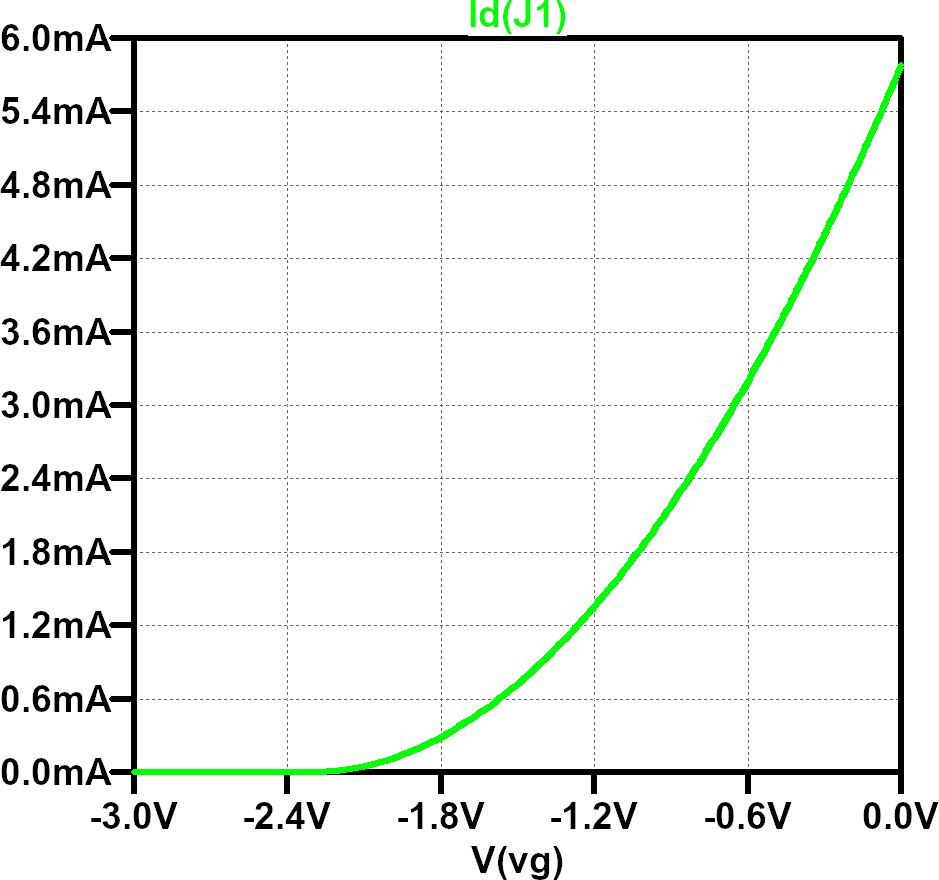
\includegraphics[width=0.8\textwidth]{images/corte-id_vgs.png}
      \caption{resultados de simulación para corte del JFET.}
      \label{fig:sim.corte}
    \end{figure}

    Para poder apreciar mejor la curva de transferencia, se redujo el barrido de la fuente hasta $3V$. Como se puede ver
    en la figura \ref{fig:sim.corte}, la tensión $V_{GS_{(OFF)}}$ se encuentra aproximadamente a los $-1.5V$. En la hoja
    de datos, el parámetro especifica un rango de entre $-0.5V$ a $-6V$, así que el modelo estaría dentro de los
    parámetros correctos.

  \section{Actividad de Laboratorio}

  \chapter{Caracteristicas de transferencia del JFET}
  En el análisis de los transistores de efecto de campo de juntura (JFET), resulta fundamental comprender la relación
  entre la tensión aplicada entre compuerta y fuente (\(V_{GS}\)) y la corriente de drenaje (\(I_D\)). Esta relación se
  conoce como característica de transferencia, ya que describe cómo la señal de entrada (voltaje de control)
  regula la corriente de salida del dispositivo.  

  La dependencia entre estas magnitudes está dada por la ecuación de Shockley, la cual permite predecir el
  comportamiento del JFET en la región de saturación. A partir de esta ecuación es posible determinar cómo varía \(I_D\)
  en función de \(V_{GS}\), estableciendo un modelo matemático que refleja el efecto de la compuerta sobre la conducción
  del canal:  

  \begin{equation}
    I_D = I_{DSS} \left( 1 - \frac{V_{GS}}{V_p} \right)^2
  \end{equation}
  
  A partir de los datos experimentales obtenidos en la curva de salida \(I_D(V_{DS})\), es posible determinar los
  valores de \(I_{DSS}\) y de la tensión de pinch-off \(V_p\). Con estos parámetros, se puede trazar la ecuación de
  Shockley y representar la característica de transferencia del JFET.  
  
  \begin{figure}[!ht]
    \centering
    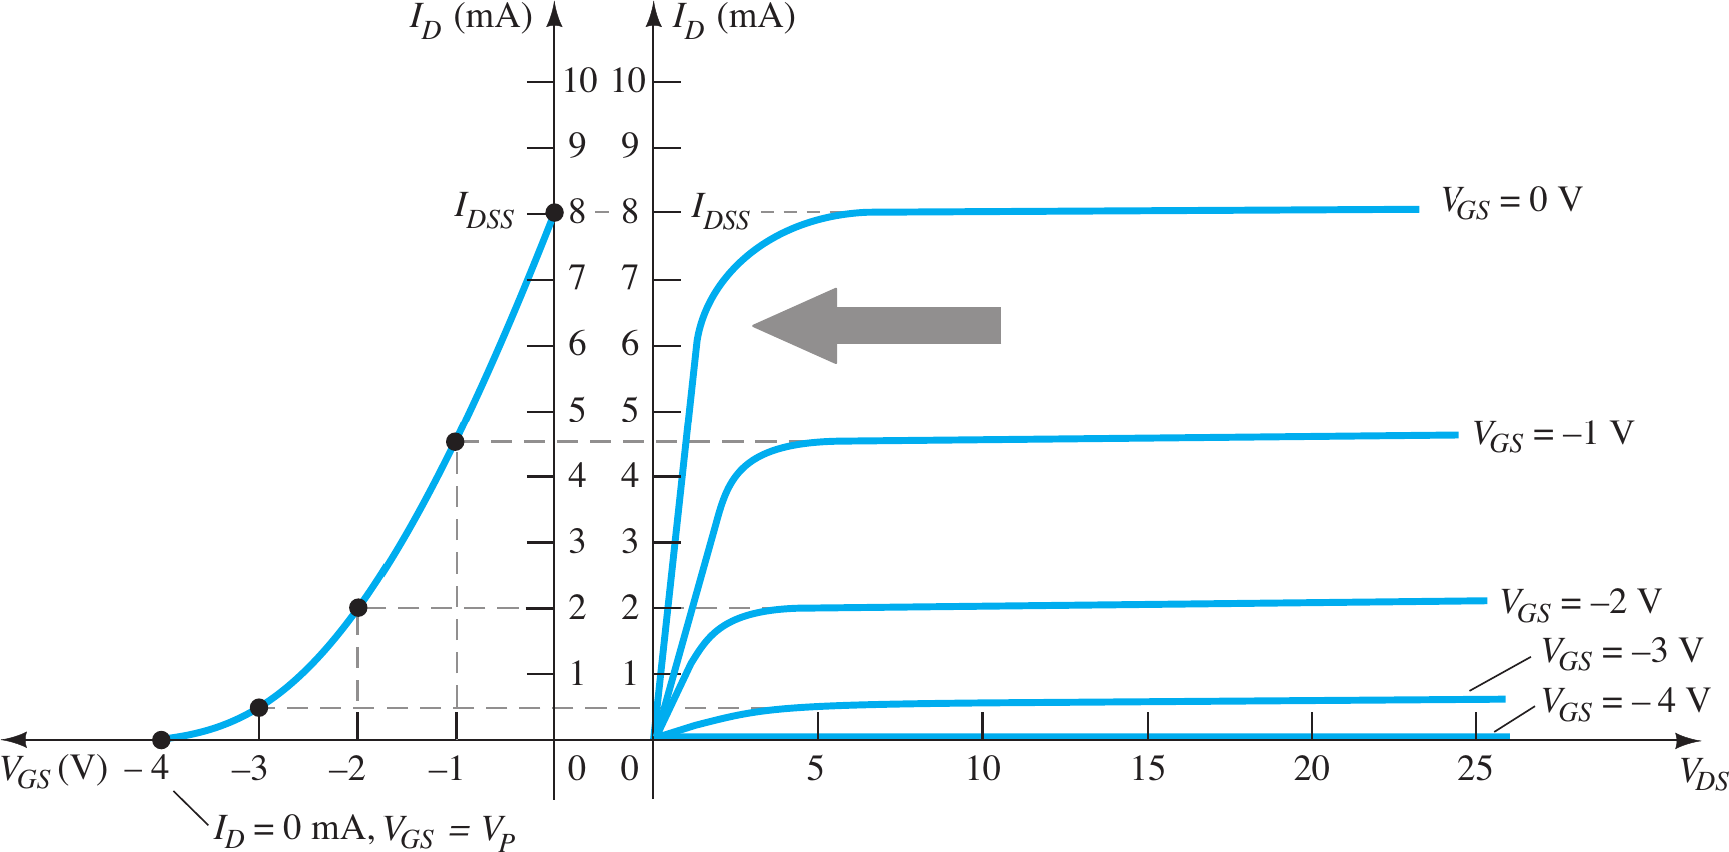
\includegraphics[width=1\textwidth]{images/grafico_transferencia.png}
    \caption{característica de transferencia del JFET obtenida a partir de la ecuación de Shockley.}
    \label{fig:transferencia}
  \end{figure}

\section{Actividad de Simulación}
    Se propuso implementar el circuito de la figura \ref{crkt:jfet-transf} en el simulador LTSpice, y hacer que la fuente
    $V1$ varíe desde $0V$ a $8V$ en pasos de $0.1V$, y por cada variacion de la fuente $V1$, que la fuente $V2$ varie de
    $0V$ a $15V$ en pasos de $0.1V$ para poder recrear una familia de curvas que expongan el comportamiento de la
    corriente $I_D$ en función del voltaje drain-source $V_{DS}$ por cada $V_{GS}$.
    \begin{figure}[!ht]
      \centering
      \begin{minipage}{0.45\textwidth}
        \begin{tikzpicture}
          % Paths, nodes and wires:
          \node[njfet](N1) at (2.25, 2.73){} node[anchor=west] at (N1.text){$BF245B$};
          \draw (4.75, 3.48) to[battery, l={$V2$}] (4.75, 1.98);
          \draw (4.75, 3.46) -- (4.75, 5.21) |- (2.25, 5.21) -| (2.25, 3.48);
          \draw (2.25, 1.96) -- (2.25, 0.73);
          \draw (4.75, 1.98) -- (4.75, 0.73);
          \node[ground] at (0.25, 0.73){};
          \node[ground] at (2.25, 0.73){};
          \node[ground] at (4.75, 0.73){};
          \draw (0.25, 1.25) to[battery, l={$V1$}] (0.25, 2);
          \draw (1.27, 2.46) -| (0.25, 2);
          \draw (0.25, 0.73) -| (0.25, 1.25);
        \end{tikzpicture}
        \caption{circuito de prueba para caracteristicas de trasnferencia.}
        \label{crkt:jfet-transf}
      \end{minipage}
      \hfill
      \begin{minipage}{0.45\textwidth}
        \begin{lstlisting}[style=ltspice, caption={Parámetros de simulación LTspice}, label=list:jfet-transf]
.MODEL  BF245B   NJF VTO = -2.3085E+000 BETA = 1.09045E-003 LAMBDA = 2.31754E-003 RD = 7.77648E+000 RS = 7.77648E+000 IS = 2.59121E-016 CGS  = 2.00000E-012 CGD  = 2.20000E-012 PB = 9.91494E-001 FC = 5.00000E-001
.dc V2 0 15 .1 V1 0 8 .1
        \end{lstlisting}
      \end{minipage}
    \end{figure}
    \begin{figure}[!ht]
      \centering
      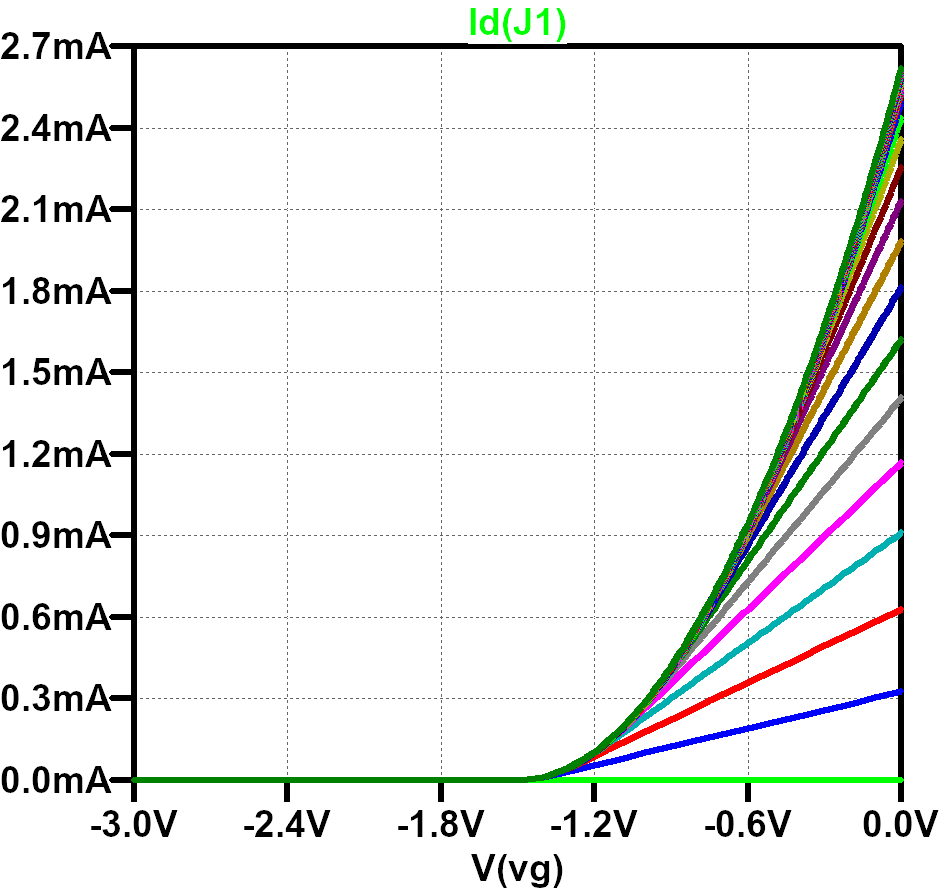
\includegraphics[width=0.8\textwidth]{images/transferencia-id_vds-vgs.png}
      \caption{resultados de simulación para caracteristicas de transferencia del JFET.}
      \label{fig:sim.transf}
    \end{figure}

    Para poder apreciar mejor los resultados de la figura \ref{fig:sim.transf}, se redujo el barrido de la fuente $V1$
    hasta $3V$ en pasos de $0.2V$. Como se puede ver, el modelo describe perfectamente la famila de curvas de
    $I_{D_{(V_{DS}, \, V_{GS}})}$. La unica diferencia observable comparada con la grafica presentada por el fabricante es el
    valor de $I_{DSS}$.

  \chapter{Interpretacion de Hojas de Datos}
En este ejercicio, se busca \textbf{familiarizarse con los parámetros más relevantes del JFET} 
leyendo su datasheet y extrayendo los valores principales a $25^\circ$C, como son:  

\begin{itemize}
    \item $I_{DSS}$: Corriente máxima de drenaje. \\ $I_{DSS} = 3mA$ 
    \item $V_{DS}$: Voltaje máximo drenaje–fuente. \\ $V_{DS} = 25V$
    \item $V_{GS}$: Voltaje máximo puerta–fuente.  \\ $V_{GS} = -2.5V$
    \item $P_D$: Potencia máxima de disipación.  \\ $P_D = 310 mW$
    \item $V_{BR}$: Voltaje de ruptura (\textit{breakdown}). \\ $V_{BR} = -25V$
    \item $V_{GS(\text{off})}$: Tensión de compuerta a la que el transistor se apaga 
    (en JFET) o umbral de corte. \\ $V_{GS(\text{off})} = -0.5V$ a $-6V$
\end{itemize}

  \chapter{Conclusiones}
Este trabajo práctico se centró en el análisis del transistor de efecto de campo de juntura (JFET), un
componente fundamental dentro de la electrónica analógica y de potencia. El JFET, por su estructura y
principio de funcionamiento, permite comprender cómo el control de una unión polarizada en inversa
afecta directamente la conducción de corriente a través de un canal semiconductor, lo que lo convierte
en un dispositivo idóneo para aplicaciones de conmutación y amplificación.  

El objetivo principal del trabajo fue caracterizar experimental y teóricamente las distintas regiones 
de operación del JFET, abarcando desde el corte hasta la saturación, así como la zona óhmica 
intermedia. Para ello, se diseñaron e implementaron circuitos en un entorno de simulación (LTSpice) 
y posteriormente se replicaron en el laboratorio utilizando instrumental básico como fuentes de 
alimentación, multímetros y protoboard.  

Durante la práctica se obtuvieron curvas características $I_{DS} = f(V_{DS})$ para diferentes valores 
de $V_{GS}$, lo que permitió observar el efecto del voltaje de compuerta sobre la corriente de drenaje. 
Asimismo, se determinó la corriente de saturación $I_{DSS}$, el voltaje de estrangulamiento 
$V_{GS(off)}$ y la característica de transferencia universal, parámetros esenciales para describir 
matemáticamente el comportamiento del dispositivo.  

La comparación entre los datos experimentales, los resultados de simulación y los valores provistos 
por el fabricante en la hoja de datos permitió no solo validar los modelos teóricos, sino también 
identificar discrepancias atribuibles a tolerancias de fabricación, condiciones de medición y 
limitaciones propias de los modelos idealizados. Esta integración entre teoría, simulación y práctica 
resulta esencial para consolidar un aprendizaje completo sobre el funcionamiento real de los 
semiconductores.   

  \chapter{Anexos}
  \section{Rubrica}
\begin{figure}[!h]
  \centering
  \begin{tabular}[c]{|c|c|c|}
    \rowcolor{gray!30}
    \hline
    \textbf{Tarea}                      & \textbf{Puntuación} & \textbf{Máximo}\\
    \hline
    Presentación del informe            &                     & 30\%\\
    \hline
    Explicación del proceso de medición &                     & 40\%\\
    \hline
    Defensa de las conclusiones         &                     & 30\%\\
    \hline
    \textbf{Total}                      &                     & \textbf{100\%}\\
    \hline
  \end{tabular}
\end{figure}

\section{Planilla de Seguimiento}
\begin{figure}[!h]
  \begin{footnotesize}
    \begin{tabular}{|m{1cm}|m{1cm}|m{1.3cm}|m{2cm}|m{1.7cm}|m{1.7cm}|m{1.7cm}|m{1.7cm}|m{1.7cm}|}
      \hline
      Versión del TP & Fecha de Inicio & Revisado Por & Resumen Observaciones Correcciones &
      Fecha de retroalimentación enviada & Cambios realizados por JTP? & Nueva fecha de entrega &
      Aprobado por jefe de cátedra?\\
      \hline
      1.0 (2025) & & & & & & &\\
      \hline
    \end{tabular}
  \end{footnotesize}
\end{figure}
 

  \section{Modelos SPICE}
    \lstinputlisting[style=ltspice, caption={Modelo SPICE del TYN612M},
    label=annex:scr_model]{simulations/models/tny612m.lib}
 
  \section{Hojas de Datos}
    \includepdf[pages=1]{annex/bt137x.pdf}
    \includepdf[pages=1]{annex/db3.pdf}
    \includepdf[pages=1]{annex/tyn612m.pdf}



\end{document}
